\section{Results and Discussion}

This large-scale microbial survey addressed the underexplored Indian Ocean, and encompassed the first microbial samples from the pristine Salomon Atoll. This was also the first large-scale ecogenomic study ever conducted aboard a private cruising yacht, with a small crew, using equipment and protocols that can be easily adapted for use aboard other sailboats. \cite{lauro_common_2014} Our study encompasses over 195 million RNA sequences and 17 million Small Subunit (SSU) ribosomal RNA tag sequences belonging to 5,264 unique Operational Taxonomic Units (OTUs), representing all three domains of life and relating to water samples spanning more than 39 degrees of latitude (Table \ref{Chagos_table1}). Data revealed the strong biogeographic partitioning present in this system and specifically identified the taxonomic drivers of shifts in microbial community composition across different oceanic regions and within the atoll.

\subfile{Chagos/table1}

\subsection{Biogeography of the Indian Ocean}

Microbial assemblages demonstrated strong biogeographic partitioning with taxonomic profiles reflecting water masses (Figures \ref{Chagos_fig1} and \ref{Chagos_fig2}). Specifically, samples from the Southern Ocean (SO), mid-latitude Southern Ocean (MSO), Bay of Bengal (BB) and Salomon Atoll (SA) formed separate, highly discrete clusters. In all cases, clustering was statistically supported using ANOSIM (global $R = 0.93$, $p < 0.05$). These results indicate that microbial assemblage composition in the Indian Ocean is influenced by the physico-chemical composition and nutrient status of oceanic water masses and that the dispersal and relative abundance of taxa may be limited by hydrodynamic boundaries of currents. \cite{brown_trait_2014} The clustering of the samples is consistent with Longhurst's marine biogeographic provinces \cite{longhurst_estimate_1995} defined using oceanographic data, measured chlorophyll, phytoplankton distributions and satellite data (Figure \ref{Chagos_fig1}, Table \ref{Chagos_table1}), further highlighting the tight coupling of microbial diversity with primary productivity and thermohaline properties. Few studies have investigated community-wide microbial biogeography in the context of Longhursts provinces, however, our results are consistent with the congruence of surface bacterioplankton communities within these regions in the eastern Atlantic Ocean. \cite{friedline_bacterial_2012} This pattern highlights the usefulness of adopting common geographical frameworks across different trophic levels and datasets to elucidate global patterns in biogeography. \cite{brown_trait_2014}

\begin{figure}
    \centering
    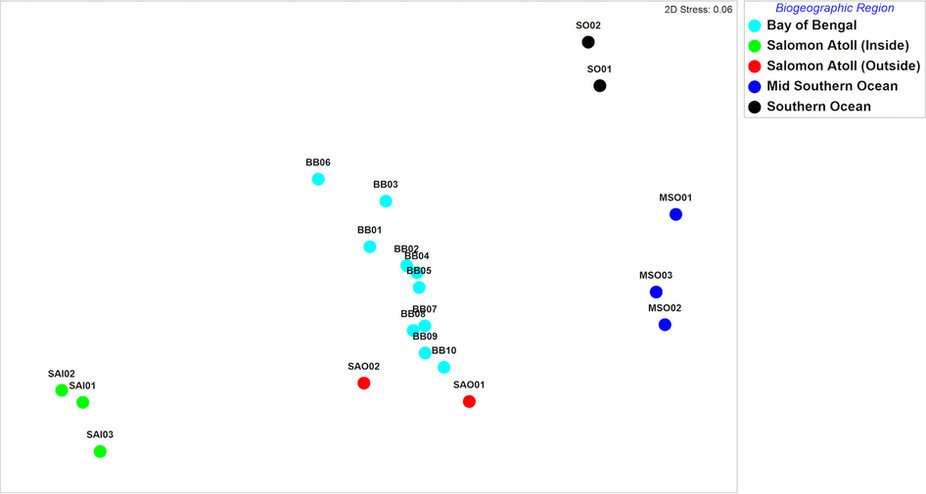
\includegraphics[width=\textwidth]{Chagos/figures/fig2}
    \caption{Bay of Bengal = BB, Salomon Atoll (inside) = SAI, Salomon Atoll (outside) = SAO, Mid-Latitude Southern Ocean = MSO, Southern Ocean = SO. ANOSIM Global $R = 0.93$.}
    \label{Chagos_fig2}
\end{figure}

Our observations of microbial provincialism are consistent with an increasing body of literature defining the discrete distributions of microbial communities in marine habitats \cite{brown_microbial_2009, agogue_water_2011, jeffries_substrate_2011, galand_unique_2009} individual marine microorganisms \cite{gomez-pereira_distinct_2010, brown_global_2012} and taxa incorporated into ocean current models. \cite{wilkins_advection_2013, hellweger_biogeographic_2014}

The key bacterial and archeal taxa driving the dissimilarity between water masses were identified by SIMPER analysis (Supplementary Table 1) with differences between water masses consistently driven by shifts in SAR11 clades, {\em Synechococcus}, and {\em Prochlorococcus}. Previous studies have shown that, within these taxa, different phylotypes show a strong biogeographic distribution. \cite{brown_trait_2014} For example, samples from the BB were differentiated from the adjacent MSO due to increased abundances of {\em Synechococcus} and decreased {\em Prochlorococcus}. Overall this biogeographic pattern resulted in different ratios of autotrophic cyanobacteria in each water mass with increased proportion of {\em Synechococcus} relative to {\em Prochlorococcus} in the BB and {\em Prochlorococcus} being 6-fold more abundant than {\em Synechococcus} in the MSO. There were also shifts in SAR11 ecotype abundance between these two water masses with the SAR11 surface clade 1b being more abundant in the MSO and the surface clade 1a being more abundant in the BB. The high degree of dissimilarity between the BB and the Southern Ocean (SO) was driven by increased abundances of SAR86, {\em Altermonas} and {\em Synechococcus} in the BB cluster relative to the SO and an increase in SAR11 clade 1b in the SO. These phylotype abundance patterns related to temperature and latitude are in agreement with the study of Brown et al. \cite{brown_global_2012} who reported that the ratio of the surface clades of SAR11 1b over 1a is highest in waters with temperatures 19–24\degree C. \cite{brown_global_2012} SAR86 similarly has a reduced genome, well-adapted to oligotrophic conditions and shows temperature driven patterns in abundance in marine metagenomes \cite{dupont_genomic_2012} with biogeographic patterns also reflecting substrate availability and niche competition with SAR11. \cite{dupont_genomic_2012} Marine {\em Synechococcus} populations display numerous phylogenetic clades and subclades \cite{mazard_multi-locus_2012} representing ecotypes adapted to a variety of environmental conditions such as temperature and nutritional requirements and which vary in abundance in tropical coastal and open ocean water masses. \cite{brown_trait_2014} Similarly the global distribution of {\em Prochlorococcus} populations is determined by temperature, nutrient concentrations and photosynthetically active radiation (PAR), with this cyanobacterium tending to dominante in more oligtrophic conditions \cite{brown_trait_2014} such as those found in the MSO.